\documentclass[letterpaper,11pt]{article}

\usepackage{latexsym}
\usepackage[empty]{fullpage}
\usepackage{titlesec}
\usepackage{marvosym}
\usepackage[usenames,dvipsnames]{color}
\usepackage{verbatim}
\usepackage{enumitem}
\usepackage[hidelinks]{hyperref}
\usepackage{fancyhdr}
\usepackage[english]{babel}
\usepackage{tabularx}
\usepackage{fontawesome5}
\usepackage{multicol}
\setlength{\multicolsep}{-3.0pt}
\setlength{\columnsep}{-1pt}
\input{glyphtounicode}

%new packages

\usepackage{fontenc}
\usepackage{amsmath}
\usepackage{amssymb}
\usepackage{graphicx}



%----------FONT OPTIONS----------

\pagestyle{fancy}
\fancyhf{} % clear all header and footer fields
\fancyfoot{}
\renewcommand{\headrulewidth}{0pt}
\renewcommand{\footrulewidth}{0pt}

% Adjust margins
\addtolength{\oddsidemargin}{-0.6in}
\addtolength{\evensidemargin}{-0.5in}
\addtolength{\textwidth}{1.19in}
\addtolength{\topmargin}{-.7in}
\addtolength{\textheight}{1.4in}

\urlstyle{same}

\raggedbottom
\raggedright
\setlength{\tabcolsep}{0in}

% Sections formatting
\titleformat{\section}{
  \vspace{-4pt}\scshape\raggedright\large\bfseries
}{}{0em}{}[\color{black}\titlerule \vspace{-5pt}]



% Ensure that generate pdf is machine readable/ATS parsable
\pdfgentounicode=1

%-------------------------
% Custom commands
\newcommand{\resumeItem}[1]{
  \item\small{
    {#1 \vspace{-2pt}}
  }
}

\newcommand{\classesList}[4]{
    \item\small{
        {#1 #2 #3 #4 \vspace{-2pt}}
  }
}

\newcommand{\resumeSubheading}[4]{
  \vspace{-2pt}\item
    \begin{tabular*}{1.0\textwidth}[t]{l@{\extracolsep{\fill}}r}
      \textbf{#1} & \textbf{\small #2} \\
      \textit{\small#3} & \textit{\small #4} \\
    \end{tabular*}\vspace{-7pt}
}

\newcommand{\resumeSubSubheading}[2]{
    \item
    \begin{tabular*}{0.97\textwidth}{l@{\extracolsep{\fill}}r}
      \textit{\small#1} & \textit{\small #2} \\
    \end{tabular*}\vspace{-7pt}
}

\newcommand{\resumeProjectHeading}[2]{
    \item
    \begin{tabular*}{1.001\textwidth}{l@{\extracolsep{\fill}}r}
      \small#1 & \textbf{\small #2}\\
    \end{tabular*}\vspace{-7pt}
}


\newcommand{\resumeSubItem}[1]{\resumeItem{#1}\vspace{-4pt}}

\renewcommand\labelitemi{$\vcenter{\hbox{\tiny$\bullet$}}$}
\renewcommand\labelitemii{$\vcenter{\hbox{\tiny$\bullet$}}$}

\newcommand{\resumeSubHeadingListStart}{\begin{itemize}[leftmargin=0.0in, label={}]}
\newcommand{\resumeSubHeadingListEnd}{\end{itemize}}
\newcommand{\resumeItemListStart}{\begin{itemize}}
\newcommand{\resumeItemListEnd}{\end{itemize}\vspace{-5pt}}


\begin{document}
\fontfamily{cmr}\selectfont
\begin{center}
\parbox{3.0cm}{%
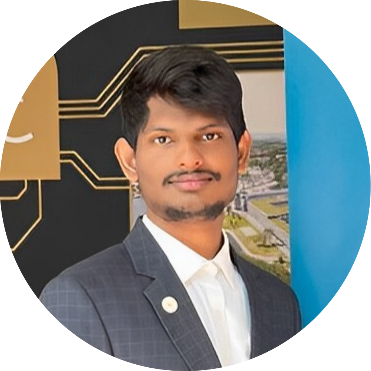
\includegraphics[width=2.7cm,clip]{images/resume_pic_m.png}}}
\parbox{\dimexpr\linewidth-3.8cm\relax}{
\vspace{-20pt}
\begin{tabularx}{\linewidth}{L r} \\
    {\Huge \scshape  Venkata Sai Yakkshit Reddy Asodi}~
    \href{https://www.cedzlabs.com/yakkshit}{\vspace{1pt}}\\
      Geneva, Switzerland. \\ \vspace{1pt}
     \small \raisebox{-0.1\height}\faPhone\ +91 8179936156 ~ \href{mailto:saiyakkshit2001@gmail.com}{\raisebox{-0.2\height}\faEnvelope\  {saiyakkshit2001@gmail.com}} ~ 
    \href{https://linkedin.com/in/yakkshit/}{\raisebox{-0.2\height}\faLinkedin\ {yakkshit}}  ~
    \href{https://yakkshit.com/}{\raisebox{-0.2\height}\faGlobe\ {yakkshit.com}}  ~
    \href{https://github.com/yakkshit}{\raisebox{-0.2\height}\faGithub{ yakkshit}}
    \vspace{-8pt}
\end{tabularx}
}
\end{center}

\vspace{-23pt}
\section{Summary \faLink}
Lead Software Engineer with a focus on AI-driven applications, Data Engineering, and full-stack development. Over 3 years of experience building scalable software solutions for large enterprises and startups. Proven expertise in cloud solutions, DevOps, and the implementation of complex data architectures.

\section{Technical Skills \faLink}
\begin{itemize}[leftmargin=0.15in, label={}]
\small{\item{
\textbf{Frontend - } React, Angular, TypeScript, Figma, Tailwind. \\
\textbf{Backend - } ASP.NET, Node.js, Python, Django. \\
\textbf{AI/ML - } LLMs, RAG, TensorFlow, GenAI. \\
\textbf{Data Engineering - } Databricks, Spark, ETL, SQL. \\
\textbf{Cloud - } AWS, Azure, CI/CD, Docker, Kubernetes. \\
\textbf{Tools - } Git, Terraform, Jenkins, JIRA.
}}
\end{itemize}

\section{Experience \faLinkedin}
\resumeSubHeadingListStart

\resumeSubheading
{Circleup AG}{Jan 2024 -- July 2024}
  {Lead Full Stack Engineer}{Zurich, Switzerland}\\
\resumeItemListStart
\resumeItem{Designed data architectures for AI applications using React, Python, and Databricks.}
\resumeItem{Developed cloud-native solutions on AWS, focusing on data pipelines and scalable APIs.}
\resumeItem{Led cross-functional teams to implement CI/CD pipelines, improving deployment efficiency.}
\resumeItemListEnd

\resumeSubheading
{cedzlabs \faBuilding}{March 2023 -- July 2024}
{Software Developer }{\faMapMarker \hspace{0.1cm} Remote, Italy.}\\
\vspace{10pt}
\resumeItemListStart
\resumeItem{I worked as a consultant to develop a software integration between Spoki and Magento. He demonstrated exceptional technical skills, professionalism, and a strong work ethic, ensuring the project was completed on time with high quality. I have effectively communicated and collaborated with our team, making a valuable asset to the project’s success.}
\end{itemize}

\section{Projects \faGithub}
\resumeSubHeadingListStart
\resumeProjectHeading
{\textbf{AI Resume Tuner} $|$ \emph{Azure, Next.js, LLMs, RAG}}{Microsoft Hackathon 2024}
\resumeItemListStart
\vspace{4pt}
\resumeItem{Developed an AI-powered resume generator that allows users to input personalized information such as skills, experience, projects, and achievements, and generate a PDF-ready resume with customizable themes. Integrated advanced features like light/dark theme toggles, section search functionality, and PDF download. Optimized the user interface with TailwindCSS and Framer Motion for seamless interactions. Incorporated functionalities for uploading resumes to LinkedIn and GitHub, improving the user experience with interactive design elements. Implemented theme combinations such as 'default,' 'google,' and 'netflix' to offer unique styles.}
\resumeItemListEnd
\vspace{4pt}
\textbf{Tools:}\emph{Nextjs, RAG, React, SQL.}
\vspace{-10pt}

\resumeProjectHeading
{\textbf{Portfolio Website} $|$ \emph{Next.js, AWS}}{Jan 2023}
\vspace{4pt}
\begin{itemize}
\item Developed and deployed a personal portfolio website on AWS using Next.js.
\item Integrated secure file storage and encryption for user uploads.
\item Designed a modern UI/UX using Figma and React.
\end{itemize}

%-----------ACHIEVEMENTS-----------
\section{Achievements}
\begin{itemize}
\item Contributed to open-source projects related to web development and cloud deployments.
\item Spearheaded the development of scalable SaaS solutions in fast-paced startup environments.
\item Active participant in hackathons and tech meetups, winning awards for innovative web applications.
\end{itemize}

\section*{Languages}
\begin{itemize}
  \item English - Fluent $|$ German - Elementary $|$ Hindi - Fluent.
\end{itemize}

\end{document}